% Created by tikzDevice version 0.12.3 on 2019-09-28 13:49:58
% !TEX encoding = UTF-8 Unicode
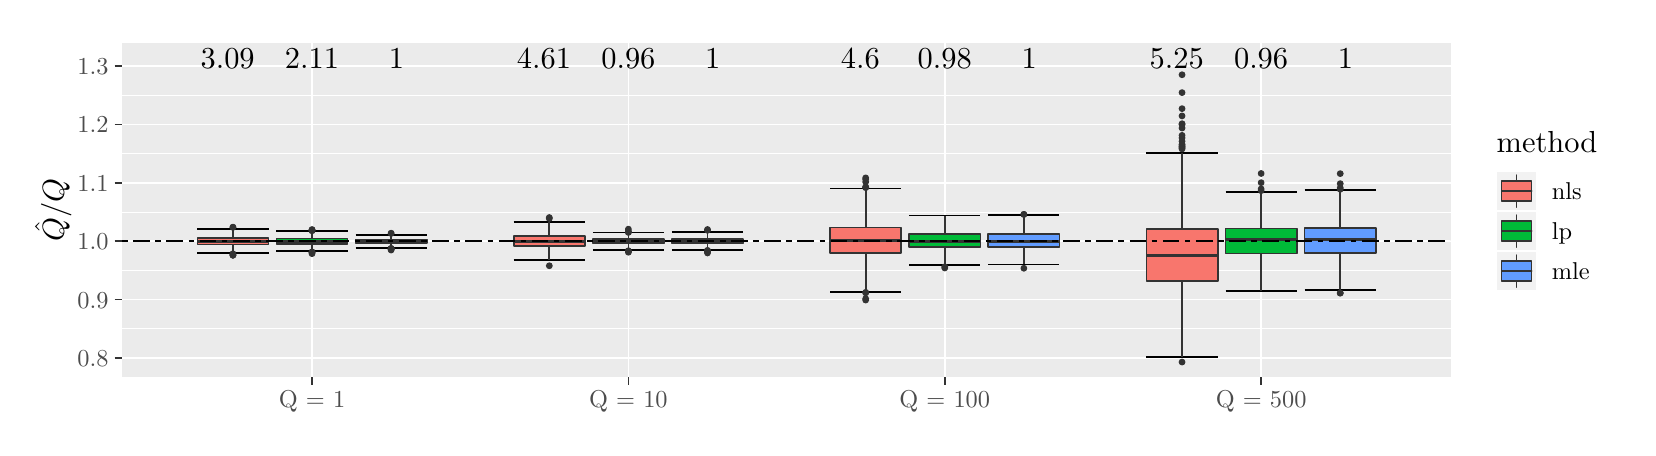
\begin{tikzpicture}[x=1pt,y=1pt]
\definecolor{fillColor}{RGB}{255,255,255}
\path[use as bounding box,fill=fillColor,fill opacity=0.00] (0,0) rectangle (578.16,144.54);
\begin{scope}
\path[clip] (  0.00,  0.00) rectangle (578.16,144.54);
\definecolor{drawColor}{RGB}{255,255,255}
\definecolor{fillColor}{RGB}{255,255,255}

\path[draw=drawColor,line width= 0.6pt,line join=round,line cap=round,fill=fillColor] (  0.00,  0.00) rectangle (578.16,144.54);
\end{scope}
\begin{scope}
\path[clip] ( 34.16, 18.22) rectangle (514.31,139.04);
\definecolor{fillColor}{gray}{0.92}

\path[fill=fillColor] ( 34.16, 18.22) rectangle (514.31,139.04);
\definecolor{drawColor}{RGB}{255,255,255}

\path[draw=drawColor,line width= 0.3pt,line join=round] ( 34.16, 35.71) --
	(514.31, 35.71);

\path[draw=drawColor,line width= 0.3pt,line join=round] ( 34.16, 56.80) --
	(514.31, 56.80);

\path[draw=drawColor,line width= 0.3pt,line join=round] ( 34.16, 77.89) --
	(514.31, 77.89);

\path[draw=drawColor,line width= 0.3pt,line join=round] ( 34.16, 98.98) --
	(514.31, 98.98);

\path[draw=drawColor,line width= 0.3pt,line join=round] ( 34.16,120.07) --
	(514.31,120.07);

\path[draw=drawColor,line width= 0.6pt,line join=round] ( 34.16, 25.17) --
	(514.31, 25.17);

\path[draw=drawColor,line width= 0.6pt,line join=round] ( 34.16, 46.26) --
	(514.31, 46.26);

\path[draw=drawColor,line width= 0.6pt,line join=round] ( 34.16, 67.35) --
	(514.31, 67.35);

\path[draw=drawColor,line width= 0.6pt,line join=round] ( 34.16, 88.43) --
	(514.31, 88.43);

\path[draw=drawColor,line width= 0.6pt,line join=round] ( 34.16,109.52) --
	(514.31,109.52);

\path[draw=drawColor,line width= 0.6pt,line join=round] ( 34.16,130.61) --
	(514.31,130.61);

\path[draw=drawColor,line width= 0.6pt,line join=round] (102.75, 18.22) --
	(102.75,139.04);

\path[draw=drawColor,line width= 0.6pt,line join=round] (217.07, 18.22) --
	(217.07,139.04);

\path[draw=drawColor,line width= 0.6pt,line join=round] (331.39, 18.22) --
	(331.39,139.04);

\path[draw=drawColor,line width= 0.6pt,line join=round] (445.71, 18.22) --
	(445.71,139.04);
\definecolor{drawColor}{RGB}{0,0,0}

\path[draw=drawColor,line width= 0.6pt,line join=round] ( 61.31, 71.77) --
	( 87.03, 71.77);

\path[draw=drawColor,line width= 0.6pt,line join=round] ( 74.17, 71.77) --
	( 74.17, 63.18);

\path[draw=drawColor,line width= 0.6pt,line join=round] ( 61.31, 63.18) --
	( 87.03, 63.18);

\path[draw=drawColor,line width= 0.6pt,line join=round] ( 89.89, 71.03) --
	(115.61, 71.03);

\path[draw=drawColor,line width= 0.6pt,line join=round] (102.75, 71.03) --
	(102.75, 63.77);

\path[draw=drawColor,line width= 0.6pt,line join=round] ( 89.89, 63.77) --
	(115.61, 63.77);

\path[draw=drawColor,line width= 0.6pt,line join=round] (118.47, 69.74) --
	(144.19, 69.74);

\path[draw=drawColor,line width= 0.6pt,line join=round] (131.33, 69.74) --
	(131.33, 64.89);

\path[draw=drawColor,line width= 0.6pt,line join=round] (118.47, 64.89) --
	(144.19, 64.89);

\path[draw=drawColor,line width= 0.6pt,line join=round] (175.63, 74.23) --
	(201.35, 74.23);

\path[draw=drawColor,line width= 0.6pt,line join=round] (188.49, 74.23) --
	(188.49, 60.50);

\path[draw=drawColor,line width= 0.6pt,line join=round] (175.63, 60.50) --
	(201.35, 60.50);

\path[draw=drawColor,line width= 0.6pt,line join=round] (204.21, 70.51) --
	(229.93, 70.51);

\path[draw=drawColor,line width= 0.6pt,line join=round] (217.07, 70.51) --
	(217.07, 64.20);

\path[draw=drawColor,line width= 0.6pt,line join=round] (204.21, 64.20) --
	(229.93, 64.20);

\path[draw=drawColor,line width= 0.6pt,line join=round] (232.79, 70.61) --
	(258.51, 70.61);

\path[draw=drawColor,line width= 0.6pt,line join=round] (245.65, 70.61) --
	(245.65, 64.12);

\path[draw=drawColor,line width= 0.6pt,line join=round] (232.79, 64.12) --
	(258.51, 64.12);

\path[draw=drawColor,line width= 0.6pt,line join=round] (289.95, 86.41) --
	(315.67, 86.41);

\path[draw=drawColor,line width= 0.6pt,line join=round] (302.81, 86.41) --
	(302.81, 49.14);

\path[draw=drawColor,line width= 0.6pt,line join=round] (289.95, 49.14) --
	(315.67, 49.14);

\path[draw=drawColor,line width= 0.6pt,line join=round] (318.53, 76.64) --
	(344.25, 76.64);

\path[draw=drawColor,line width= 0.6pt,line join=round] (331.39, 76.64) --
	(331.39, 58.67);

\path[draw=drawColor,line width= 0.6pt,line join=round] (318.53, 58.67) --
	(344.25, 58.67);

\path[draw=drawColor,line width= 0.6pt,line join=round] (347.11, 76.93) --
	(372.83, 76.93);

\path[draw=drawColor,line width= 0.6pt,line join=round] (359.97, 76.93) --
	(359.97, 59.01);

\path[draw=drawColor,line width= 0.6pt,line join=round] (347.11, 59.01) --
	(372.83, 59.01);

\path[draw=drawColor,line width= 0.6pt,line join=round] (404.27, 99.28) --
	(430.00, 99.28);

\path[draw=drawColor,line width= 0.6pt,line join=round] (417.13, 99.28) --
	(417.13, 25.46);

\path[draw=drawColor,line width= 0.6pt,line join=round] (404.27, 25.46) --
	(430.00, 25.46);

\path[draw=drawColor,line width= 0.6pt,line join=round] (432.85, 85.10) --
	(458.58, 85.10);

\path[draw=drawColor,line width= 0.6pt,line join=round] (445.71, 85.10) --
	(445.71, 49.43);

\path[draw=drawColor,line width= 0.6pt,line join=round] (432.85, 49.43) --
	(458.58, 49.43);

\path[draw=drawColor,line width= 0.6pt,line join=round] (461.43, 85.78) --
	(487.16, 85.78);

\path[draw=drawColor,line width= 0.6pt,line join=round] (474.29, 85.78) --
	(474.29, 49.64);

\path[draw=drawColor,line width= 0.6pt,line join=round] (461.43, 49.64) --
	(487.16, 49.64);
\definecolor{drawColor}{gray}{0.20}
\definecolor{fillColor}{gray}{0.20}

\path[draw=drawColor,line width= 0.4pt,line join=round,line cap=round,fill=fillColor] ( 74.17, 62.33) circle (  1.02);

\path[draw=drawColor,line width= 0.4pt,line join=round,line cap=round,fill=fillColor] ( 74.17, 62.33) circle (  1.02);

\path[draw=drawColor,line width= 0.4pt,line join=round,line cap=round,fill=fillColor] ( 74.17, 62.85) circle (  1.02);

\path[draw=drawColor,line width= 0.4pt,line join=round,line cap=round,fill=fillColor] ( 74.17, 72.46) circle (  1.02);

\path[draw=drawColor,line width= 0.4pt,line join=round,line cap=round,fill=fillColor] ( 74.17, 62.38) circle (  1.02);

\path[draw=drawColor,line width= 0.4pt,line join=round,line cap=round,fill=fillColor] ( 74.17, 72.39) circle (  1.02);

\path[draw=drawColor,line width= 0.6pt,line join=round] ( 74.17, 68.49) -- ( 74.17, 71.77);

\path[draw=drawColor,line width= 0.6pt,line join=round] ( 74.17, 66.24) -- ( 74.17, 63.18);
\definecolor{fillColor}{RGB}{248,118,109}

\path[draw=drawColor,line width= 0.6pt,line join=round,line cap=round,fill=fillColor] ( 61.31, 68.49) --
	( 61.31, 66.24) --
	( 87.03, 66.24) --
	( 87.03, 68.49) --
	( 61.31, 68.49) --
	cycle;

\path[draw=drawColor,line width= 1.1pt,line join=round] ( 61.31, 67.35) -- ( 87.03, 67.35);
\definecolor{fillColor}{gray}{0.20}

\path[draw=drawColor,line width= 0.4pt,line join=round,line cap=round,fill=fillColor] (102.75, 62.88) circle (  1.02);

\path[draw=drawColor,line width= 0.4pt,line join=round,line cap=round,fill=fillColor] (102.75, 63.26) circle (  1.02);

\path[draw=drawColor,line width= 0.4pt,line join=round,line cap=round,fill=fillColor] (102.75, 71.18) circle (  1.02);

\path[draw=drawColor,line width= 0.4pt,line join=round,line cap=round,fill=fillColor] (102.75, 63.43) circle (  1.02);

\path[draw=drawColor,line width= 0.4pt,line join=round,line cap=round,fill=fillColor] (102.75, 71.53) circle (  1.02);

\path[draw=drawColor,line width= 0.4pt,line join=round,line cap=round,fill=fillColor] (102.75, 63.49) circle (  1.02);

\path[draw=drawColor,line width= 0.4pt,line join=round,line cap=round,fill=fillColor] (102.75, 71.55) circle (  1.02);

\path[draw=drawColor,line width= 0.4pt,line join=round,line cap=round,fill=fillColor] (102.75, 71.19) circle (  1.02);

\path[draw=drawColor,line width= 0.6pt,line join=round] (102.75, 68.31) -- (102.75, 71.03);

\path[draw=drawColor,line width= 0.6pt,line join=round] (102.75, 66.47) -- (102.75, 63.77);
\definecolor{fillColor}{RGB}{0,186,56}

\path[draw=drawColor,line width= 0.6pt,line join=round,line cap=round,fill=fillColor] ( 89.89, 68.31) --
	( 89.89, 66.47) --
	(115.61, 66.47) --
	(115.61, 68.31) --
	( 89.89, 68.31) --
	cycle;

\path[draw=drawColor,line width= 1.1pt,line join=round] ( 89.89, 67.35) -- (115.61, 67.35);
\definecolor{fillColor}{gray}{0.20}

\path[draw=drawColor,line width= 0.4pt,line join=round,line cap=round,fill=fillColor] (131.33, 64.18) circle (  1.02);

\path[draw=drawColor,line width= 0.4pt,line join=round,line cap=round,fill=fillColor] (131.33, 70.25) circle (  1.02);

\path[draw=drawColor,line width= 0.4pt,line join=round,line cap=round,fill=fillColor] (131.33, 64.66) circle (  1.02);

\path[draw=drawColor,line width= 0.4pt,line join=round,line cap=round,fill=fillColor] (131.33, 64.55) circle (  1.02);

\path[draw=drawColor,line width= 0.4pt,line join=round,line cap=round,fill=fillColor] (131.33, 70.21) circle (  1.02);

\path[draw=drawColor,line width= 0.4pt,line join=round,line cap=round,fill=fillColor] (131.33, 64.53) circle (  1.02);

\path[draw=drawColor,line width= 0.4pt,line join=round,line cap=round,fill=fillColor] (131.33, 64.65) circle (  1.02);

\path[draw=drawColor,line width= 0.4pt,line join=round,line cap=round,fill=fillColor] (131.33, 64.79) circle (  1.02);

\path[draw=drawColor,line width= 0.4pt,line join=round,line cap=round,fill=fillColor] (131.33, 64.64) circle (  1.02);

\path[draw=drawColor,line width= 0.6pt,line join=round] (131.33, 67.97) -- (131.33, 69.74);

\path[draw=drawColor,line width= 0.6pt,line join=round] (131.33, 66.70) -- (131.33, 64.89);
\definecolor{fillColor}{RGB}{97,156,255}

\path[draw=drawColor,line width= 0.6pt,line join=round,line cap=round,fill=fillColor] (118.47, 67.97) --
	(118.47, 66.70) --
	(144.19, 66.70) --
	(144.19, 67.97) --
	(118.47, 67.97) --
	cycle;

\path[draw=drawColor,line width= 1.1pt,line join=round] (118.47, 67.35) -- (144.19, 67.35);
\definecolor{fillColor}{gray}{0.20}

\path[draw=drawColor,line width= 0.4pt,line join=round,line cap=round,fill=fillColor] (188.49, 58.51) circle (  1.02);

\path[draw=drawColor,line width= 0.4pt,line join=round,line cap=round,fill=fillColor] (188.49, 75.93) circle (  1.02);

\path[draw=drawColor,line width= 0.4pt,line join=round,line cap=round,fill=fillColor] (188.49, 75.57) circle (  1.02);

\path[draw=drawColor,line width= 0.6pt,line join=round] (188.49, 69.32) -- (188.49, 74.23);

\path[draw=drawColor,line width= 0.6pt,line join=round] (188.49, 65.54) -- (188.49, 60.50);
\definecolor{fillColor}{RGB}{248,118,109}

\path[draw=drawColor,line width= 0.6pt,line join=round,line cap=round,fill=fillColor] (175.63, 69.32) --
	(175.63, 65.54) --
	(201.35, 65.54) --
	(201.35, 69.32) --
	(175.63, 69.32) --
	cycle;

\path[draw=drawColor,line width= 1.1pt,line join=round] (175.63, 67.44) -- (201.35, 67.44);
\definecolor{fillColor}{gray}{0.20}

\path[draw=drawColor,line width= 0.4pt,line join=round,line cap=round,fill=fillColor] (217.07, 63.91) circle (  1.02);

\path[draw=drawColor,line width= 0.4pt,line join=round,line cap=round,fill=fillColor] (217.07, 63.40) circle (  1.02);

\path[draw=drawColor,line width= 0.4pt,line join=round,line cap=round,fill=fillColor] (217.07, 70.59) circle (  1.02);

\path[draw=drawColor,line width= 0.4pt,line join=round,line cap=round,fill=fillColor] (217.07, 63.61) circle (  1.02);

\path[draw=drawColor,line width= 0.4pt,line join=round,line cap=round,fill=fillColor] (217.07, 70.95) circle (  1.02);

\path[draw=drawColor,line width= 0.4pt,line join=round,line cap=round,fill=fillColor] (217.07, 63.83) circle (  1.02);

\path[draw=drawColor,line width= 0.4pt,line join=round,line cap=round,fill=fillColor] (217.07, 71.74) circle (  1.02);

\path[draw=drawColor,line width= 0.4pt,line join=round,line cap=round,fill=fillColor] (217.07, 70.63) circle (  1.02);

\path[draw=drawColor,line width= 0.6pt,line join=round] (217.07, 68.12) -- (217.07, 70.51);

\path[draw=drawColor,line width= 0.6pt,line join=round] (217.07, 66.50) -- (217.07, 64.20);
\definecolor{fillColor}{RGB}{0,186,56}

\path[draw=drawColor,line width= 0.6pt,line join=round,line cap=round,fill=fillColor] (204.21, 68.12) --
	(204.21, 66.50) --
	(229.93, 66.50) --
	(229.93, 68.12) --
	(204.21, 68.12) --
	cycle;

\path[draw=drawColor,line width= 1.1pt,line join=round] (204.21, 67.30) -- (229.93, 67.30);
\definecolor{fillColor}{gray}{0.20}

\path[draw=drawColor,line width= 0.4pt,line join=round,line cap=round,fill=fillColor] (245.65, 63.68) circle (  1.02);

\path[draw=drawColor,line width= 0.4pt,line join=round,line cap=round,fill=fillColor] (245.65, 64.02) circle (  1.02);

\path[draw=drawColor,line width= 0.4pt,line join=round,line cap=round,fill=fillColor] (245.65, 63.74) circle (  1.02);

\path[draw=drawColor,line width= 0.4pt,line join=round,line cap=round,fill=fillColor] (245.65, 63.13) circle (  1.02);

\path[draw=drawColor,line width= 0.4pt,line join=round,line cap=round,fill=fillColor] (245.65, 71.32) circle (  1.02);

\path[draw=drawColor,line width= 0.4pt,line join=round,line cap=round,fill=fillColor] (245.65, 64.01) circle (  1.02);

\path[draw=drawColor,line width= 0.4pt,line join=round,line cap=round,fill=fillColor] (245.65, 71.61) circle (  1.02);

\path[draw=drawColor,line width= 0.6pt,line join=round] (245.65, 68.14) -- (245.65, 70.61);

\path[draw=drawColor,line width= 0.6pt,line join=round] (245.65, 66.49) -- (245.65, 64.12);
\definecolor{fillColor}{RGB}{97,156,255}

\path[draw=drawColor,line width= 0.6pt,line join=round,line cap=round,fill=fillColor] (232.79, 68.14) --
	(232.79, 66.49) --
	(258.51, 66.49) --
	(258.51, 68.14) --
	(232.79, 68.14) --
	cycle;

\path[draw=drawColor,line width= 1.1pt,line join=round] (232.79, 67.34) -- (258.51, 67.34);
\definecolor{fillColor}{gray}{0.20}

\path[draw=drawColor,line width= 0.4pt,line join=round,line cap=round,fill=fillColor] (302.81, 48.72) circle (  1.02);

\path[draw=drawColor,line width= 0.4pt,line join=round,line cap=round,fill=fillColor] (302.81, 88.80) circle (  1.02);

\path[draw=drawColor,line width= 0.4pt,line join=round,line cap=round,fill=fillColor] (302.81, 48.89) circle (  1.02);

\path[draw=drawColor,line width= 0.4pt,line join=round,line cap=round,fill=fillColor] (302.81, 86.77) circle (  1.02);

\path[draw=drawColor,line width= 0.4pt,line join=round,line cap=round,fill=fillColor] (302.81, 46.12) circle (  1.02);

\path[draw=drawColor,line width= 0.4pt,line join=round,line cap=round,fill=fillColor] (302.81, 86.82) circle (  1.02);

\path[draw=drawColor,line width= 0.4pt,line join=round,line cap=round,fill=fillColor] (302.81, 90.26) circle (  1.02);

\path[draw=drawColor,line width= 0.4pt,line join=round,line cap=round,fill=fillColor] (302.81, 46.60) circle (  1.02);

\path[draw=drawColor,line width= 0.4pt,line join=round,line cap=round,fill=fillColor] (302.81, 89.78) circle (  1.02);

\path[draw=drawColor,line width= 0.4pt,line join=round,line cap=round,fill=fillColor] (302.81, 87.00) circle (  1.02);

\path[draw=drawColor,line width= 0.6pt,line join=round] (302.81, 72.39) -- (302.81, 86.41);

\path[draw=drawColor,line width= 0.6pt,line join=round] (302.81, 63.00) -- (302.81, 49.14);
\definecolor{fillColor}{RGB}{248,118,109}

\path[draw=drawColor,line width= 0.6pt,line join=round,line cap=round,fill=fillColor] (289.95, 72.39) --
	(289.95, 63.00) --
	(315.67, 63.00) --
	(315.67, 72.39) --
	(289.95, 72.39) --
	cycle;

\path[draw=drawColor,line width= 1.1pt,line join=round] (289.95, 67.68) -- (315.67, 67.68);
\definecolor{fillColor}{gray}{0.20}

\path[draw=drawColor,line width= 0.4pt,line join=round,line cap=round,fill=fillColor] (331.39, 58.13) circle (  1.02);

\path[draw=drawColor,line width= 0.4pt,line join=round,line cap=round,fill=fillColor] (331.39, 57.70) circle (  1.02);

\path[draw=drawColor,line width= 0.6pt,line join=round] (331.39, 69.91) -- (331.39, 76.64);

\path[draw=drawColor,line width= 0.6pt,line join=round] (331.39, 65.24) -- (331.39, 58.67);
\definecolor{fillColor}{RGB}{0,186,56}

\path[draw=drawColor,line width= 0.6pt,line join=round,line cap=round,fill=fillColor] (318.53, 69.91) --
	(318.53, 65.24) --
	(344.25, 65.24) --
	(344.25, 69.91) --
	(318.53, 69.91) --
	cycle;

\path[draw=drawColor,line width= 1.1pt,line join=round] (318.53, 67.39) -- (344.25, 67.39);
\definecolor{fillColor}{gray}{0.20}

\path[draw=drawColor,line width= 0.4pt,line join=round,line cap=round,fill=fillColor] (359.97, 57.61) circle (  1.02);

\path[draw=drawColor,line width= 0.4pt,line join=round,line cap=round,fill=fillColor] (359.97, 77.07) circle (  1.02);

\path[draw=drawColor,line width= 0.4pt,line join=round,line cap=round,fill=fillColor] (359.97, 77.07) circle (  1.02);

\path[draw=drawColor,line width= 0.6pt,line join=round] (359.97, 69.94) -- (359.97, 76.93);

\path[draw=drawColor,line width= 0.6pt,line join=round] (359.97, 65.26) -- (359.97, 59.01);
\definecolor{fillColor}{RGB}{97,156,255}

\path[draw=drawColor,line width= 0.6pt,line join=round,line cap=round,fill=fillColor] (347.11, 69.94) --
	(347.11, 65.26) --
	(372.83, 65.26) --
	(372.83, 69.94) --
	(347.11, 69.94) --
	cycle;

\path[draw=drawColor,line width= 1.1pt,line join=round] (347.11, 67.35) -- (372.83, 67.35);
\definecolor{fillColor}{gray}{0.20}

\path[draw=drawColor,line width= 0.4pt,line join=round,line cap=round,fill=fillColor] (417.13,104.71) circle (  1.02);

\path[draw=drawColor,line width= 0.4pt,line join=round,line cap=round,fill=fillColor] (417.13,127.53) circle (  1.02);

\path[draw=drawColor,line width= 0.4pt,line join=round,line cap=round,fill=fillColor] (417.13,101.06) circle (  1.02);

\path[draw=drawColor,line width= 0.4pt,line join=round,line cap=round,fill=fillColor] (417.13,101.45) circle (  1.02);

\path[draw=drawColor,line width= 0.4pt,line join=round,line cap=round,fill=fillColor] (417.13,109.83) circle (  1.02);

\path[draw=drawColor,line width= 0.4pt,line join=round,line cap=round,fill=fillColor] (417.13,115.28) circle (  1.02);

\path[draw=drawColor,line width= 0.4pt,line join=round,line cap=round,fill=fillColor] (417.13, 23.71) circle (  1.02);

\path[draw=drawColor,line width= 0.4pt,line join=round,line cap=round,fill=fillColor] (417.13,112.65) circle (  1.02);

\path[draw=drawColor,line width= 0.4pt,line join=round,line cap=round,fill=fillColor] (417.13,105.63) circle (  1.02);

\path[draw=drawColor,line width= 0.4pt,line join=round,line cap=round,fill=fillColor] (417.13,108.27) circle (  1.02);

\path[draw=drawColor,line width= 0.4pt,line join=round,line cap=round,fill=fillColor] (417.13,109.55) circle (  1.02);

\path[draw=drawColor,line width= 0.4pt,line join=round,line cap=round,fill=fillColor] (417.13,121.08) circle (  1.02);

\path[draw=drawColor,line width= 0.4pt,line join=round,line cap=round,fill=fillColor] (417.13,101.64) circle (  1.02);

\path[draw=drawColor,line width= 0.4pt,line join=round,line cap=round,fill=fillColor] (417.13,103.47) circle (  1.02);

\path[draw=drawColor,line width= 0.4pt,line join=round,line cap=round,fill=fillColor] (417.13,102.09) circle (  1.02);

\path[draw=drawColor,line width= 0.4pt,line join=round,line cap=round,fill=fillColor] (417.13,100.72) circle (  1.02);

\path[draw=drawColor,line width= 0.4pt,line join=round,line cap=round,fill=fillColor] (417.13,102.38) circle (  1.02);

\path[draw=drawColor,line width= 0.6pt,line join=round] (417.13, 71.88) -- (417.13, 99.28);

\path[draw=drawColor,line width= 0.6pt,line join=round] (417.13, 52.95) -- (417.13, 25.46);
\definecolor{fillColor}{RGB}{248,118,109}

\path[draw=drawColor,line width= 0.6pt,line join=round,line cap=round,fill=fillColor] (404.27, 71.88) --
	(404.27, 52.95) --
	(430.00, 52.95) --
	(430.00, 71.88) --
	(404.27, 71.88) --
	cycle;

\path[draw=drawColor,line width= 1.1pt,line join=round] (404.27, 62.10) -- (430.00, 62.10);
\definecolor{fillColor}{gray}{0.20}

\path[draw=drawColor,line width= 0.4pt,line join=round,line cap=round,fill=fillColor] (445.71, 85.64) circle (  1.02);

\path[draw=drawColor,line width= 0.4pt,line join=round,line cap=round,fill=fillColor] (445.71, 91.85) circle (  1.02);

\path[draw=drawColor,line width= 0.4pt,line join=round,line cap=round,fill=fillColor] (445.71, 88.53) circle (  1.02);

\path[draw=drawColor,line width= 0.4pt,line join=round,line cap=round,fill=fillColor] (445.71, 86.28) circle (  1.02);

\path[draw=drawColor,line width= 0.6pt,line join=round] (445.71, 72.03) -- (445.71, 85.10);

\path[draw=drawColor,line width= 0.6pt,line join=round] (445.71, 62.99) -- (445.71, 49.43);
\definecolor{fillColor}{RGB}{0,186,56}

\path[draw=drawColor,line width= 0.6pt,line join=round,line cap=round,fill=fillColor] (432.85, 72.03) --
	(432.85, 62.99) --
	(458.58, 62.99) --
	(458.58, 72.03) --
	(432.85, 72.03) --
	cycle;

\path[draw=drawColor,line width= 1.1pt,line join=round] (432.85, 67.86) -- (458.58, 67.86);
\definecolor{fillColor}{gray}{0.20}

\path[draw=drawColor,line width= 0.4pt,line join=round,line cap=round,fill=fillColor] (474.29, 86.66) circle (  1.02);

\path[draw=drawColor,line width= 0.4pt,line join=round,line cap=round,fill=fillColor] (474.29, 48.62) circle (  1.02);

\path[draw=drawColor,line width= 0.4pt,line join=round,line cap=round,fill=fillColor] (474.29, 48.65) circle (  1.02);

\path[draw=drawColor,line width= 0.4pt,line join=round,line cap=round,fill=fillColor] (474.29, 91.80) circle (  1.02);

\path[draw=drawColor,line width= 0.4pt,line join=round,line cap=round,fill=fillColor] (474.29, 86.14) circle (  1.02);

\path[draw=drawColor,line width= 0.4pt,line join=round,line cap=round,fill=fillColor] (474.29, 88.18) circle (  1.02);

\path[draw=drawColor,line width= 0.6pt,line join=round] (474.29, 72.24) -- (474.29, 85.78);

\path[draw=drawColor,line width= 0.6pt,line join=round] (474.29, 63.00) -- (474.29, 49.64);
\definecolor{fillColor}{RGB}{97,156,255}

\path[draw=drawColor,line width= 0.6pt,line join=round,line cap=round,fill=fillColor] (461.43, 72.24) --
	(461.43, 63.00) --
	(487.16, 63.00) --
	(487.16, 72.24) --
	(461.43, 72.24) --
	cycle;

\path[draw=drawColor,line width= 1.1pt,line join=round] (461.43, 67.84) -- (487.16, 67.84);
\definecolor{drawColor}{RGB}{0,0,0}

\path[draw=drawColor,line width= 0.6pt,dash pattern=on 2pt off 2pt on 6pt off 2pt ,line join=round] ( 34.16, 67.35) -- (514.31, 67.35);

\node[text=drawColor,anchor=base,inner sep=0pt, outer sep=0pt, scale=  1.10] at (133.23,129.75) {1};

\node[text=drawColor,anchor=base,inner sep=0pt, outer sep=0pt, scale=  1.10] at (102.75,129.75) {2.11};

\node[text=drawColor,anchor=base,inner sep=0pt, outer sep=0pt, scale=  1.10] at ( 72.26,129.75) {3.09};

\node[text=drawColor,anchor=base,inner sep=0pt, outer sep=0pt, scale=  1.10] at (247.56,129.75) {1};

\node[text=drawColor,anchor=base,inner sep=0pt, outer sep=0pt, scale=  1.10] at (217.07,129.75) {0.96};

\node[text=drawColor,anchor=base,inner sep=0pt, outer sep=0pt, scale=  1.10] at (186.59,129.75) {4.61};

\node[text=drawColor,anchor=base,inner sep=0pt, outer sep=0pt, scale=  1.10] at (361.88,129.75) {1};

\node[text=drawColor,anchor=base,inner sep=0pt, outer sep=0pt, scale=  1.10] at (331.39,129.75) {0.98};

\node[text=drawColor,anchor=base,inner sep=0pt, outer sep=0pt, scale=  1.10] at (300.91,129.75) {4.6};

\node[text=drawColor,anchor=base,inner sep=0pt, outer sep=0pt, scale=  1.10] at (476.20,129.75) {1};

\node[text=drawColor,anchor=base,inner sep=0pt, outer sep=0pt, scale=  1.10] at (445.71,129.75) {0.96};

\node[text=drawColor,anchor=base,inner sep=0pt, outer sep=0pt, scale=  1.10] at (415.23,129.75) {5.25};
\end{scope}
\begin{scope}
\path[clip] (  0.00,  0.00) rectangle (578.16,144.54);
\definecolor{drawColor}{gray}{0.30}

\node[text=drawColor,anchor=base east,inner sep=0pt, outer sep=0pt, scale=  0.88] at ( 29.21, 22.14) {0.8};

\node[text=drawColor,anchor=base east,inner sep=0pt, outer sep=0pt, scale=  0.88] at ( 29.21, 43.23) {0.9};

\node[text=drawColor,anchor=base east,inner sep=0pt, outer sep=0pt, scale=  0.88] at ( 29.21, 64.32) {1.0};

\node[text=drawColor,anchor=base east,inner sep=0pt, outer sep=0pt, scale=  0.88] at ( 29.21, 85.40) {1.1};

\node[text=drawColor,anchor=base east,inner sep=0pt, outer sep=0pt, scale=  0.88] at ( 29.21,106.49) {1.2};

\node[text=drawColor,anchor=base east,inner sep=0pt, outer sep=0pt, scale=  0.88] at ( 29.21,127.58) {1.3};
\end{scope}
\begin{scope}
\path[clip] (  0.00,  0.00) rectangle (578.16,144.54);
\definecolor{drawColor}{gray}{0.20}

\path[draw=drawColor,line width= 0.6pt,line join=round] ( 31.41, 25.17) --
	( 34.16, 25.17);

\path[draw=drawColor,line width= 0.6pt,line join=round] ( 31.41, 46.26) --
	( 34.16, 46.26);

\path[draw=drawColor,line width= 0.6pt,line join=round] ( 31.41, 67.35) --
	( 34.16, 67.35);

\path[draw=drawColor,line width= 0.6pt,line join=round] ( 31.41, 88.43) --
	( 34.16, 88.43);

\path[draw=drawColor,line width= 0.6pt,line join=round] ( 31.41,109.52) --
	( 34.16,109.52);

\path[draw=drawColor,line width= 0.6pt,line join=round] ( 31.41,130.61) --
	( 34.16,130.61);
\end{scope}
\begin{scope}
\path[clip] (  0.00,  0.00) rectangle (578.16,144.54);
\definecolor{drawColor}{gray}{0.20}

\path[draw=drawColor,line width= 0.6pt,line join=round] (102.75, 15.47) --
	(102.75, 18.22);

\path[draw=drawColor,line width= 0.6pt,line join=round] (217.07, 15.47) --
	(217.07, 18.22);

\path[draw=drawColor,line width= 0.6pt,line join=round] (331.39, 15.47) --
	(331.39, 18.22);

\path[draw=drawColor,line width= 0.6pt,line join=round] (445.71, 15.47) --
	(445.71, 18.22);
\end{scope}
\begin{scope}
\path[clip] (  0.00,  0.00) rectangle (578.16,144.54);
\definecolor{drawColor}{gray}{0.30}

\node[text=drawColor,anchor=base,inner sep=0pt, outer sep=0pt, scale=  0.88] at (102.75,  7.21) {Q = 1};

\node[text=drawColor,anchor=base,inner sep=0pt, outer sep=0pt, scale=  0.88] at (217.07,  7.21) {Q = 10};

\node[text=drawColor,anchor=base,inner sep=0pt, outer sep=0pt, scale=  0.88] at (331.39,  7.21) {Q = 100};

\node[text=drawColor,anchor=base,inner sep=0pt, outer sep=0pt, scale=  0.88] at (445.71,  7.21) {Q = 500};
\end{scope}
\begin{scope}
\path[clip] (  0.00,  0.00) rectangle (578.16,144.54);
\definecolor{drawColor}{RGB}{0,0,0}

\node[text=drawColor,rotate= 90.00,anchor=base,inner sep=0pt, outer sep=0pt, scale=  1.10] at ( 13.08, 78.63) {$\hat{Q}/Q$};
\end{scope}
\begin{scope}
\path[clip] (  0.00,  0.00) rectangle (578.16,144.54);
\definecolor{fillColor}{RGB}{255,255,255}

\path[fill=fillColor] (525.31, 43.84) rectangle (572.66,113.42);
\end{scope}
\begin{scope}
\path[clip] (  0.00,  0.00) rectangle (578.16,144.54);
\definecolor{drawColor}{RGB}{0,0,0}

\node[text=drawColor,anchor=base west,inner sep=0pt, outer sep=0pt, scale=  1.10] at (530.81, 99.27) {method};
\end{scope}
\begin{scope}
\path[clip] (  0.00,  0.00) rectangle (578.16,144.54);
\definecolor{drawColor}{RGB}{255,255,255}
\definecolor{fillColor}{gray}{0.95}

\path[draw=drawColor,line width= 0.6pt,line join=round,line cap=round,fill=fillColor] (530.81, 78.25) rectangle (545.26, 92.70);
\end{scope}
\begin{scope}
\path[clip] (  0.00,  0.00) rectangle (578.16,144.54);
\definecolor{drawColor}{gray}{0.20}

\path[draw=drawColor,line width= 0.6pt,line join=round,line cap=round] (538.03, 79.70) --
	(538.03, 81.86);

\path[draw=drawColor,line width= 0.6pt,line join=round,line cap=round] (538.03, 89.09) --
	(538.03, 91.26);
\definecolor{fillColor}{RGB}{248,118,109}

\path[draw=drawColor,line width= 0.6pt,line join=round,line cap=round,fill=fillColor] (532.61, 81.86) rectangle (543.45, 89.09);

\path[draw=drawColor,line width= 0.6pt,line join=round,line cap=round] (532.61, 85.48) --
	(543.45, 85.48);
\end{scope}
\begin{scope}
\path[clip] (  0.00,  0.00) rectangle (578.16,144.54);
\definecolor{drawColor}{RGB}{255,255,255}
\definecolor{fillColor}{gray}{0.95}

\path[draw=drawColor,line width= 0.6pt,line join=round,line cap=round,fill=fillColor] (530.81, 63.80) rectangle (545.26, 78.25);
\end{scope}
\begin{scope}
\path[clip] (  0.00,  0.00) rectangle (578.16,144.54);
\definecolor{drawColor}{gray}{0.20}

\path[draw=drawColor,line width= 0.6pt,line join=round,line cap=round] (538.03, 65.24) --
	(538.03, 67.41);

\path[draw=drawColor,line width= 0.6pt,line join=round,line cap=round] (538.03, 74.64) --
	(538.03, 76.81);
\definecolor{fillColor}{RGB}{0,186,56}

\path[draw=drawColor,line width= 0.6pt,line join=round,line cap=round,fill=fillColor] (532.61, 67.41) rectangle (543.45, 74.64);

\path[draw=drawColor,line width= 0.6pt,line join=round,line cap=round] (532.61, 71.02) --
	(543.45, 71.02);
\end{scope}
\begin{scope}
\path[clip] (  0.00,  0.00) rectangle (578.16,144.54);
\definecolor{drawColor}{RGB}{255,255,255}
\definecolor{fillColor}{gray}{0.95}

\path[draw=drawColor,line width= 0.6pt,line join=round,line cap=round,fill=fillColor] (530.81, 49.34) rectangle (545.26, 63.80);
\end{scope}
\begin{scope}
\path[clip] (  0.00,  0.00) rectangle (578.16,144.54);
\definecolor{drawColor}{gray}{0.20}

\path[draw=drawColor,line width= 0.6pt,line join=round,line cap=round] (538.03, 50.79) --
	(538.03, 52.96);

\path[draw=drawColor,line width= 0.6pt,line join=round,line cap=round] (538.03, 60.18) --
	(538.03, 62.35);
\definecolor{fillColor}{RGB}{97,156,255}

\path[draw=drawColor,line width= 0.6pt,line join=round,line cap=round,fill=fillColor] (532.61, 52.96) rectangle (543.45, 60.18);

\path[draw=drawColor,line width= 0.6pt,line join=round,line cap=round] (532.61, 56.57) --
	(543.45, 56.57);
\end{scope}
\begin{scope}
\path[clip] (  0.00,  0.00) rectangle (578.16,144.54);
\definecolor{drawColor}{RGB}{0,0,0}

\node[text=drawColor,anchor=base west,inner sep=0pt, outer sep=0pt, scale=  0.88] at (550.76, 82.45) {nls};
\end{scope}
\begin{scope}
\path[clip] (  0.00,  0.00) rectangle (578.16,144.54);
\definecolor{drawColor}{RGB}{0,0,0}

\node[text=drawColor,anchor=base west,inner sep=0pt, outer sep=0pt, scale=  0.88] at (550.76, 67.99) {lp};
\end{scope}
\begin{scope}
\path[clip] (  0.00,  0.00) rectangle (578.16,144.54);
\definecolor{drawColor}{RGB}{0,0,0}

\node[text=drawColor,anchor=base west,inner sep=0pt, outer sep=0pt, scale=  0.88] at (550.76, 53.54) {mle};
\end{scope}
\end{tikzpicture}
